

\documentclass[journal]{IEEEtran}
% Paquete para importar imágenes
\usepackage{graphicx}  
\usepackage[spanish]{babel}
\usepackage{float}
\ifCLASSINFOpdf
  % \usepackage[pdftex]{graphicx}
  % declare the path(s) where your graphic files are
  % \graphicspath{{../pdf/}{../jpeg/}}
  % and their extensions so you won't have to specify these with
  % every instance of \includegraphics
  % \DeclareGraphicsExtensions{.pdf,.jpeg,.png}
\else
  % or other class option (dvipsone, dvipdf, if not using dvips). graphicx
  % will default to the driver specified in the system graphics.cfg if no
  % driver is specified.
  % \usepackage[dvips]{graphicx}
  % declare the path(s) where your graphic files are
  % \graphicspath{{../eps/}}
  % and their extensions so you won't have to specify these with
  % every instance of \includegraphics
  % \DeclareGraphicsExtensions{.eps}
\fi
% graphicx was written by David Carlisle and Sebastian Rahtz. It is
% required if you want graphics, photos, etc. graphicx.sty is already
% installed on most LaTeX systems. The latest version and documentation
% can be obtained at: 
% http://www.ctan.org/pkg/graphicx
% Another good source of documentation is "Using Imported Graphics in
% LaTeX2e" by Keith Reckdahl which can be found at:
% http://www.ctan.org/pkg/epslatex
%
% latex, and pdflatex in dvi mode, support graphics in encapsulated
% postscript (.eps) format. pdflatex in pdf mode supports graphics
% in .pdf, .jpeg, .png and .mps (metapost) formats. Users should ensure
% that all non-photo figures use a vector format (.eps, .pdf, .mps) and
% not a bitmapped formats (.jpeg, .png). The IEEE frowns on bitmapped formats
% which can result in "jaggedy"/blurry rendering of lines and letters as
% well as large increases in file sizes.
%
% You can find documentation about the pdfTeX application at:
% http://www.tug.org/applications/pdftex





% *** MATH PACKAGES ***
%
\usepackage{amsmath}
% A popular package from the American Mathematical Society that provides
% many useful and powerful commands for dealing with mathematics.
%
% Note that the amsmath package sets \interdisplaylinepenalty to 10000
% thus preventing page breaks from occurring within multiline equations. Use:
%\interdisplaylinepenalty=2500
% after loading amsmath to restore such page breaks as IEEEtran.cls normally
% does. amsmath.sty is already installed on most LaTeX systems. The latest
% version and documentation can be obtained at:
% http://www.ctan.org/pkg/amsmath





% *** SPECIALIZED LIST PACKAGES ***
%
\usepackage{algorithmic}
% algorithmic.sty was written by Peter Williams and Rogerio Brito.
% This package provides an algorithmic environment fo describing algorithms.
% You can use the algorithmic environment in-text or within a figure
% environment to provide for a floating algorithm. Do NOT use the algorithm
% floating environment provided by algorithm.sty (by the same authors) or
% algorithm2e.sty (by Christophe Fiorio) as the IEEE does not use dedicated
% algorithm float types and packages that provide these will not provide
% correct IEEE style captions. The latest version and documentation of
% algorithmic.sty can be obtained at:
% http://www.ctan.org/pkg/algorithms
% Also of interest may be the (relatively newer and more customizable)
% algorithmicx.sty package by Szasz Janos:
% http://www.ctan.org/pkg/algorithmicx




% *** ALIGNMENT PACKAGES ***
%
%\usepackage{array}
% Frank Mittelbach's and David Carlisle's array.sty patches and improves
% the standard LaTeX2e array and tabular environments to provide better
% appearance and additional user controls. As the default LaTeX2e table
% generation code is lacking to the point of almost being broken with
% respect to the quality of the end results, all users are strongly
% advised to use an enhanced (at the very least that provided by array.sty)
% set of table tools. array.sty is already installed on most systems. The
% latest version and documentation can be obtained at:
% http://www.ctan.org/pkg/array


% IEEEtran contains the IEEEeqnarray family of commands that can be used to
% generate multiline equations as well as matrices, tables, etc., of high
% quality.




% *** SUBFIGURE PACKAGES ***
%\ifCLASSOPTIONcompsoc
%  \usepackage[caption=false,font=normalsize,labelfont=sf,textfont=sf]{subfig}
%\else
%  \usepackage[caption=false,font=footnotesize]{subfig}
%\fi
% subfig.sty, written by Steven Douglas Cochran, is the modern replacement
% for subfigure.sty, the latter of which is no longer maintained and is
% incompatible with some LaTeX packages including fixltx2e. However,
% subfig.sty requires and automatically loads Axel Sommerfeldt's caption.sty
% which will override IEEEtran.cls' handling of captions and this will result
% in non-IEEE style figure/table captions. To prevent this problem, be sure
% and invoke subfig.sty's "caption=false" package option (available since
% subfig.sty version 1.3, 2005/06/28) as this is will preserve IEEEtran.cls
% handling of captions.
% Note that the Computer Society format requires a larger sans serif font
% than the serif footnote size font used in traditional IEEE formatting
% and thus the need to invoke different subfig.sty package options depending
% on whether compsoc mode has been enabled.
%
% The latest version and documentation of subfig.sty can be obtained at:
% http://www.ctan.org/pkg/subfig




% *** FLOAT PACKAGES ***
%
%\usepackage{fixltx2e}
% fixltx2e, the successor to the earlier fix2col.sty, was written by
% Frank Mittelbach and David Carlisle. This package corrects a few problems
% in the LaTeX2e kernel, the most notable of which is that in current
% LaTeX2e releases, the ordering of single and double column floats is not
% guaranteed to be preserved. Thus, an unpatched LaTeX2e can allow a
% single column figure to be placed prior to an earlier double column
% figure.
% Be aware that LaTeX2e kernels dated 2015 and later have fixltx2e.sty's
% corrections already built into the system in which case a warning will
% be issued if an attempt is made to load fixltx2e.sty as it is no longer
% needed.
% The latest version and documentation can be found at:
% http://www.ctan.org/pkg/fixltx2e


%\usepackage{stfloats}
% stfloats.sty was written by Sigitas Tolusis. This package gives LaTeX2e
% the ability to do double column floats at the bottom of the page as well
% as the top. (e.g., "\begin{figure*}[!b]" is not normally possible in
% LaTeX2e). It also provides a command:
%\fnbelowfloat
% to enable the placement of footnotes below bottom floats (the standard
% LaTeX2e kernel puts them above bottom floats). This is an invasive package
% which rewrites many portions of the LaTeX2e float routines. It may not work
% with other packages that modify the LaTeX2e float routines. The latest
% version and documentation can be obtained at:
% http://www.ctan.org/pkg/stfloats
% Do not use the stfloats baselinefloat ability as the IEEE does not allow
% \baselineskip to stretch. Authors submitting work to the IEEE should note
% that the IEEE rarely uses double column equations and that authors should try
% to avoid such use. Do not be tempted to use the cuted.sty or midfloat.sty
% packages (also by Sigitas Tolusis) as the IEEE does not format its papers in
% such ways.
% Do not attempt to use stfloats with fixltx2e as they are incompatible.
% Instead, use Morten Hogholm'a dblfloatfix which combines the features
% of both fixltx2e and stfloats:
%
% \usepackage{dblfloatfix}
% The latest version can be found at:
% http://www.ctan.org/pkg/dblfloatfix




%\ifCLASSOPTIONcaptionsoff
%  \usepackage[nomarkers]{endfloat}
% \let\MYoriglatexcaption\caption
% \renewcommand{\caption}[2][\relax]{\MYoriglatexcaption[#2]{#2}}
%\fi
% endfloat.sty was written by James Darrell McCauley, Jeff Goldberg and 
% Axel Sommerfeldt. This package may be useful when used in conjunction with 
% IEEEtran.cls'  captionsoff option. Some IEEE journals/societies require that
% submissions have lists of figures/tables at the end of the paper and that
% figures/tables without any captions are placed on a page by themselves at
% the end of the document. If needed, the draftcls IEEEtran class option or
% \CLASSINPUTbaselinestretch interface can be used to increase the line
% spacing as well. Be sure and use the nomarkers option of endfloat to
% prevent endfloat from "marking" where the figures would have been placed
% in the text. The two hack lines of code above are a slight modification of
% that suggested by in the endfloat docs (section 8.4.1) to ensure that
% the full captions always appear in the list of figures/tables - even if
% the user used the short optional argument of \caption[]{}.
% IEEE papers do not typically make use of \caption[]'s optional argument,
% so this should not be an issue. A similar trick can be used to disable
% captions of packages such as subfig.sty that lack options to turn off
% the subcaptions:
% For subfig.sty:
% \let\MYorigsubfloat\subfloat
% \renewcommand{\subfloat}[2][\relax]{\MYorigsubfloat[]{#2}}
% However, the above trick will not work if both optional arguments of
% the \subfloat command are used. Furthermore, there needs to be a
% description of each subfigure *somewhere* and endfloat does not add
% subfigure captions to its list of figures. Thus, the best approach is to
% avoid the use of subfigure captions (many IEEE journals avoid them anyway)
% and instead reference/explain all the subfigures within the main caption.
% The latest version of endfloat.sty and its documentation can obtained at:
% http://www.ctan.org/pkg/endfloat
%
% The IEEEtran \ifCLASSOPTIONcaptionsoff conditional can also be used
% later in the document, say, to conditionally put the References on a 
% page by themselves.




% *** PDF, URL AND HYPERLINK PACKAGES ***
%
%\usepackage{url}
% url.sty was written by Donald Arseneau. It provides better support for
% handling and breaking URLs. url.sty is already installed on most LaTeX
% systems. The latest version and documentation can be obtained at:
% http://www.ctan.org/pkg/url
% Basically, \url{my_url_here}.




% *** Do not adjust lengths that control margins, column widths, etc. ***
% *** Do not use packages that alter fonts (such as pslatex).         ***
% There should be no need to do such things with IEEEtran.cls V1.6 and later.
% (Unless specifically asked to do so by the journal or conference you plan
% to submit to, of course. )


% correct bad hyphenation here
\hyphenation{op-tical net-works semi-conduc-tor}


\begin{document}
%
% paper title
% Titles are generally capitalized except for words such as a, an, and, as,
% at, but, by, for, in, nor, of, on, or, the, to and up, which are usually
% not capitalized unless they are the first or last word of the title.
% Linebreaks \\ can be used within to get better formatting as desired.
% Do not put math or special symbols in the title.
\title{Control predictivo GPC para un motor DC}
%
%
% author names and IEEE memberships
% note positions of commas and nonbreaking spaces ( ~ ) LaTeX will not break
% a structure at a ~ so this keeps an author's name from being broken across
% two lines.
% use \thanks{} to gain access to the first footnote area
% a separate \thanks must be used for each paragraph as LaTeX2e's \thanks
% was not built to handle multiple paragraphs
%

\author{\IEEEauthorblockN{Rodrigo Salazar, Elvin Soto, Carlos Fuhrhop}

\IEEEauthorblockA{Escuela de graduados\\
Universidad Austral de Chile (UACh)}}
%\thanks{M. Shell was with the Department of Electrical and Computer Engineering, %Georgia Institute of Technology, Atlanta, GA, 30332 USA e-mail: (see %http://www.michaelshell.org/contact.html).}
%\thanks{J. Doe and J. Doe are with Anonymous University.}
%\thanks{Manuscript received April 19, 2005; revised August 26, 2015.}}

% note the % following the last \IEEEmembership and also \thanks - 
% these prevent an unwanted space from occurring between the last author name
% and the end of the author line. i.e., if you had this:
% 
% \author{....lastname \thanks{...} \thanks{...} }
%                     ^------------^------------^----Do not want these spaces!
%
% a space would be appended to the last name and could cause every name on that
% line to be shifted left slightly. This is one of those "LaTeX things". For
% instance, "\textbf{A} \textbf{B}" will typeset as "A B" not "AB". To get
% "AB" then you have to do: "\textbf{A}\textbf{B}"
% \thanks is no different in this regard, so shield the last } of each \thanks
% that ends a line with a % and do not let a space in before the next \thanks.
% Spaces after \IEEEmembership other than the last one are OK (and needed) as
% you are supposed to have spaces between the names. For what it is worth,
% this is a minor point as most people would not even notice if the said evil
% space somehow managed to creep in.



% The paper headers
%\markboth{Journal of \LaTeX\ Class Files,~Vol.~14, No.~8, August~2015}%
\markboth{Control Avanzado ELEL315-21, ENERO 2024}
{Shell \MakeLowercase{\textit{et al.}}: Bare Demo of IEEEtran.cls for IEEE Journals}
% The only time the second header will appear is for the odd numbered pages
% after the title page when using the twoside option.
% 
% *** Note that you probably will NOT want to include the author's ***
% *** name in the headers of peer review papers.                   ***
% You can use \ifCLASSOPTIONpeerreview for conditional compilation here if
% you desire.




% If you want to put a publisher's ID mark on the page you can do it like
% this:
%\IEEEpubid{0000--0000/00\$00.00~\copyright~2015 IEEE}
% Remember, if you use this you must call \IEEEpubidadjcol in the second
% column for its text to clear the IEEEpubid mark.



% use for special paper notices
%\IEEEspecialpapernotice{(Invited Paper)}

% make the title area
\maketitle

% As a general rule, do not put math, special symbols or citations
% in the abstract or keywords.
\begin{abstract}
Este trabajo aborda la aplicación de una estrategia de control avanzada, conocida como Control Predictivo Generalizado (GPC) para un circuito de motor de corriente continua (DC). Se presenta una revisión del modelo del motor DC y del modelo de control predicitivo  del GPC para adaptarse al comportamiento dinámico del motor DC. Los resultados se desarrollan en un ambiente de simulacion usando el lenguaje de programación Python y se muestra el comportamiento del modelo en términos de seguimiento de referencia. Este enfoque ofrece una perspectiva para el control de sistemas en aplicaciones prácticas, destacando el potencial del Control Predictivo Generalizado en el ámbito de los motores de corriente continua.
\end{abstract}

% Note that keywords are not normally used for peerreview papers.
\begin{IEEEkeywords}
Control GPC, Motor DC.
\end{IEEEkeywords}


% For peer review papers, you can put extra information on the cover
% page as needed:
% \ifCLASSOPTIONpeerreview
% \begin{center} \bfseries EDICS Category: 3-BBND \end{center}
% \fi
%
% For peerreview papers, this IEEEtran command inserts a page break and
% creates the second title. It will be ignored for other modes.
\IEEEpeerreviewmaketitle



\section{Introducción}


\IEEEPARstart{E}l control de un motor de corriente continua (DC) se realiza con el objetivo de regular su velocidad, dirección y/o par motor a partir de una entrada que generalmete es una fuente de voltaje [1]. Estos motores son ampliamente utilizados en diversas aplicaciones debido a su capacidad para ofrecer un control preciso sobre estos parámetros. En este trabajo, nos enfocaremos en una estrategia de control predictivo específica conocida como Control Predictivo Generalizado (GPC, por sus siglas en inglés), explorando cómo esta técnica busca alcanzar el objetivo de control, como por ejemplo la regulación de velocidad rotacional que se abordará a lo largo del presente.
El trabajo se dividirá en dos secciones. En primer lugar se explicará el modelo matemático del motor DC y la matriz de espacio-estado generada y también la estrategia control GPC y en segundo lugar se analizarán los resultados de la estrategia aplicada.



\section{Desarrollo}


\subsection{Descripción del modelo}
El motor de corriente directa (DC) ha sido usado por muchos años como un convertidor básico de energía, es decir, convierte energía eléctrica en energía mecánica. Estos motores son usados en procesos industriales como elevadores eléctricos, laminadores, vehículos eléctricos y algunas bombas donde se requiere de velocidad variable [3].

\begin{figure}[h]
    \centering
    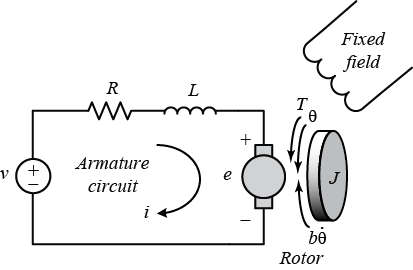
\includegraphics[width=1\linewidth]{motor.png}
    \caption{Esquema de un circuito de motor DC}
    \label{fig:enter-label}
\end{figure}

El motor DC se modela con una resistencia constante R en serie con una inductancia constante L que representa la inductancia de la bobina del rotor, y una fuente de alimentación $v$ que representa el voltaje generado en el rotor.

Si se analiza la malla en el circuito se obtiene lo siguiente:

\begin{equation*}
    v(t)= Ri(t) + L\frac{di(t)}{dt}+E_a (t), 
\end{equation*}
\\
Despejando para $L\frac{di(t)}{dt}$ queda:
\begin{align}
 L\frac{di(t)}{dt} &= v(t)-Ri(t) - E_a (t), 
\end{align}

Las pérdidas por fricción y parte de la energía desarrollada es almacenada como energía cinética en la masa que gira del rotor. La ecuación de la sección mecánica viene dada por el modelo:

\begin{equation*}
    T_m(t) = J\frac{d\omega(t)}{dt}+B\omega(t), 
\end{equation*}
\\
Despejando para $J\frac{d\omega(t)}{dt}$ queda:
\begin{align}
 J\frac{d\omega(t)}{dt} &= T_m(t)-B\omega(t), 
\end{align}

La ecuación anterior surge del balance de momento en el motor donde $T_m(t)$ es el torque del motor de corriente continua, $B$ es el coeficiente de fricción equivalente al motor de CD y la carga montados sobre el eje del motor, J es el momento de inercia total del rotor y de la carga con relación al eje del motor, $\omega(t)$ es la velocidad angular del motor y $\dfrac{d\omega(t)}{dt}$ es la aceleración angular.

Para poder lograr la interacción entre las ecuaciones anteriores se proponen las siguientes relaciones que asumen que existe una relación proporcional, $K_a$ (Constante de fuerza contraelectromotriz $[v/rad s]$), entre el voltaje inducido en la armadura y la velocidad angular del eje del motor.

\begin{align}
E_a(t) &= K_a\omega(t),
\end{align}

Y se supone la siguiente relación electromecánica que establece que el torque mecánico es proporcional, $K_m$ (Constante de Torque $[Nm / A]$), a la corriente eléctrica que circula por el motor DC.

\begin{align}
T_m(t) &= K_m i(t),
\end{align}

\subsection{Función de transferencia del sistema}

Al aplicar la transformada de laplace a las ecuaciones anteriores tenemos:
\begin{align}
Lsi(s) &= v(s)-Ri(s)-E_a(s), \\
Js\omega(s) &= T_m(s)-B\omega(s), \\
E_a(s)) &=K_a\omega(s), \\
T_m(s)) &=K_mi(s), 
\end{align}

Sustituyendo la ecuación 7 y 8 en la ecuación 5 queda:

\begin{align}
Ls\frac{T_m}{K_m} &= v(s)-R\frac{T_m}{K_m}-K_a\omega(s), \\
v(s)&=\frac{(R+Ls)T_m}{K_m}+K_a\omega(s),
\end{align}

De la ecuación 6 calculamos la velocidad angular
\begin{align}
\omega(s)=\frac{T_m}{Js+B}
\end{align}

Sustituyendo la ecuación 12 en la ecuación 11 nos queda:\\
\begin{align}
v(s)&=\frac{(R+Ls)T_m}{K_m}+K_a\frac{T_m}{Js+B}\\
v(s)&=(\frac{R+Ls}{K_m}+\frac{k_a}{Js+B}T_m\\
v(s)&=\frac{(R+Ls)(Js+BT)+k_a k_m}{K_m(Js+B)}T_m,
\end{align}
\\
De esta forma podemos obtener la función de transferencia que relaciona la salida (torque)  del motor de CD con la entrada (voltaje)

\begin{align}
\frac{T_m(s)}{v(s)}&=\frac{K_m(Js+B)}{LJs^2+(RJ+LB)s+RB+K_m K_a}
\end{align}

Es importante mencionar que este sistema se puede expresar en función de varias salidas. De la misma forma, se pueden usar las ecuaciones para obtener la función de transferencia que relacionan cualquier salida con la entrada que es el voltaje.

Función de transferencia de la fuerza contraelectromotriz con relación al voltaje:

\begin{align}
\frac{E_a(s)}{v(s)}&=\frac{K_m K_a}{LJs^2+(RJ+LB)s+RB+K_m K_a}
\end{align}
\\
Función de transferencia de la corriente del rotor con relación al voltaje:

\begin{align}
\frac{i(s)}{v(s)}&=\frac{Js+B}{LJs^2+(RJ+LB)s+RB+K_m K_a}
\end{align}

Función de transferencia de la velocidad angular con relación al voltaje:

\begin{align}
\frac{\omega(s)}{v(s)}&=\frac{K_m}{LJs^2+(RJ+LB)s+RB+K_m K_a}
\end{align}

Por otro lado si estamos interesados en conocer la posición del motor de corriente directa DC, basta simplemente con integrar la velocidad angular, en otras palabras, simplemente colocamos un integrador a la función de transferencia anterior. Por lo tanto la ecuación que representa la posición del Motor DC es:

\begin{align}
\frac{\theta(s)}{v(s)}&=\frac{K_m}{s(LJs^2+(RJ+LB)s+RB+K_m K_a)}
\end{align}

\subsection{Espacio estado}
Definimos los estados como:

\begin{align}
x_1&=\omega \\
\dot{x}_1&=\dot{\omega} \\
x_2&=i \\
\dot{x}_2&=\dot{i} 
\end{align}

Reescribiendo las ecuaciones se tiene:

\begin{align}
\dot{x}_1&=-\frac{B}{J}x_1+\frac{K_m}{J}x_2 \\
\dot{x}_2&=-\frac{R}{L}x_2+\frac{K_a}{L}x_1+\frac{1}{L}v
\end{align}
\\
Lo anterior se hace tomando las ecuaciones 1 y 2 donde se  sustituye tmabién la ecuación 3 y 4. 
La representación del modelo del motor DC en espacio estado [1] en forma matricial es:
\[
\begin{bmatrix}
    \dot{x}_1 \\
    \dot{x}_2 \\
\end{bmatrix}
=
\begin{bmatrix}
    -\frac{B}{J} & \frac{K_m}{J} \\
    -\frac{K_a}{L} & -\frac{R}{L} \\
\end{bmatrix}
\begin{bmatrix}
    x_1 \\
    x_2 \\
\end{bmatrix}
+
\begin{bmatrix}
    0 \\
    \frac{1}{L} \\
\end{bmatrix} v
\]
\\
Reemplazando los valores del cuadro 1 queda:
\[
\begin{bmatrix}
    \dot{x}_1 \\
    \dot{x}_2 \\
\end{bmatrix}
=
\begin{bmatrix}
    -10 & 1 \\
    -0.02 & -2 \\
\end{bmatrix}
\begin{bmatrix}
    x_1 \\
    x_2 \\
\end{bmatrix}
+
\begin{bmatrix}
    0 \\
    2 \\
\end{bmatrix} v
\]

\subsection{Datos del modelo}
\begin{table}[htbp]
    \centering
    \caption{Parámetros del motor DC [1]}
    \begin{tabular}{|c|c|c|c|c|c|}
        \hline
        Momento de inercia del rotor (J) & 0.01 $kg.m^2$ \\
        \hline
        Constante de amortiguamiento del motor & 0.1 N.m.s  \\
        \hline
        Constante de rotor FEM (Fuerza electromotriz ($K_c$) & 0.01 V/rad/sec  \\
        \hline
        Constante de torque de motor ($k_t$) & 0.01 N.m/Amp \\
        \hline
        Resistencia de rotor (R) & 1 Ohm \\
        \hline
         Inductancia de rotor (L) & 0.5 H \\
        \hline
    \end{tabular}
\end{table}

\subsection{Control Predictivo Generalizado (GPC)}
Para implementar un controlador GPC, primero se definen los parámetros y matrices del modelo del sistema que deseamos controlar. El modelo mostrado por Huang en espacio de estados está dado por las siguientes ecuaciones [2]:

\begin{align}
x(t + 1) &= Ax(t) + Bu(t),\label{eq:sistema1} \\
y(t) &= Hx(t) \label{eq:sistema2}
\end{align}

El criterio de rendimiento \( J \) es:


\begin{align*}
J = &\frac{1}{2} \sum_{j=1}^{p_1} [y_d(t + j) - \hat{y}(t + j)]^T Q_j [y_d(t + j) - \hat{y}(t + j)] \\
& + \frac{1}{2} \sum_{j=0}^{p_2} \Delta u(t + j)^T R_j \Delta u(t + j),
\end{align*}


O también descrita para un intervalo de predicción:

\begin{align}
J = \frac{1}{2} \left[ (Y_d - Y)^T Q (Y_d - Y) + \Delta U^T R \Delta U \right],
\end{align}

Donde \( Y_d \) es el vector de referencia deseado, \( Y \) la salida predicha,  \(Q\) la matriz de ponderación del error y \( R \) la matriz de ponderación respecto al esfuerzo de control. Este criterio de desempeño se utiliza en muchos controladores predictivos. Para tratar con incrementos de control en lugar de la salida de control, la ecuación compuesta puede escribirse como:

\begin{align}
Y = Gx(t) + F_{11} \Delta U + F_2 u(t - 1)
\end{align}

Donde:

\[
G = 
\begin{bmatrix}
HA \\
HA^2 \\
\vdots \\
HA^{p_1}
\end{bmatrix},
\]

\[
F_{11} = \begin{bmatrix}
    HB & 0 & \cdots & 0 \\
    H(A + I)B & HB & \cdots & 0 \\
    \vdots & \vdots & \ddots & \vdots \\
    H\varUpsilon(p_2)B & H\varUpsilon(p_2 - 1)B & \cdots & H(A^{p_1 - p_2 - 1}B)
\end{bmatrix},
\]

\[
F_2 = \begin{bmatrix}
    HB \\
    H(A + I)B \\
    \vdots \\
    H(A^{p1 - 1} + A^{p1 - 2} + \ldots + A^{p2 - p1 - 1})B
\end{bmatrix},
\]

\[
\Delta U = [\Delta u(t), \Delta u(t + 1), \ldots, \Delta u(t + p_2)]^T
\]

Con \[
\varUpsilon(j) = \sum_{k=0}^{j} A^{p_{1} - p_{2} - 1 + k}
\]


La solución para el cambio en la señal de control \( \Delta U \) que minimiza \( J \) es:
\begin{align}\label{ecua-control}
\Delta U = (F_{11}^T Q F_{11} + rI)^{-1} F_{11}^T Q \left[Y_d - Gx(t) - F_2 u(t - 1)\right]
\end{align}

Aunque (\ref{ecua-control}) proporciona la secuencia de control completa que minimiza \( J \) en el horizonte de predicción, solo se aplican al sistema los valores de las primeras \( m \) filas como la señal de control. Por lo tanto, la ley de control final tiene la forma:

\begin{align}
\Delta u(t) = g_1 [Y_d - Gx(t) - F_2u(t - 1)]
\end{align}

Con \( g_1 = \left[ I_m, 0, 0, \ldots, 0 \right] \left( F_{11}^T Q F_{11} + R \right)^{-1} F_{11}^T Q \), siendo \( F_{11}^T Q \) las primeras \( m \) filas de la matriz \( \left( F_{11}^T Q F_{11} + R \right)^{-1} F_{11}^T Q \). \\

Para implementar un controlador Predictivo Basado en Modelo (GPC) en Python, sigue los siguientes pasos:

\begin{enumerate}
    \item Define el modelo del sistema. Establece las matrices \( A \), \( B \), y \( H \) según el modelo de tu sistema.
    \item Calcula las matrices \( G \), \( F_{11} \) y \( F_2 \) con base en las matrices del sistema y los horizontes de predicción y control.
    \item Define la función objetivo \( J \) que incluye el seguimiento de la referencia y el esfuerzo de control, con matrices de ponderación \( Q \) y \( R \).
    \item Optimiza \( J \) respecto a la secuencia de control \( \Delta U \), sujeto a las restricciones del sistema, para calcular el control óptimo en cada paso de tiempo.
\end{enumerate}

Los parámetros definidos en el modelo son:

\begin{table} [htbp]
    \centering
    \caption{Parámetros del modelo GPC [1]}
    \begin{tabular}{|c|c|c|c|c|c|}
        \hline
        Horizonte de predicción ($p_1$) & 5  \\
        \hline
        Horizonte de control ($p_2$) & 3  \\
        \hline
        Valor matriz de peso Q & 9  \\
        \hline
        Valor matriz de peso R & 0.5 \\
        \hline
       
    \end{tabular}
\end{table}


\section{Experiencia práctica}
\subsection{Discretización del modelo}
Para discretizar el modelo, fue utilizado el metodo de Euler hacia adelante (Forward Euler). Dado el modelo de espacio-estado presentadas en las ecuaciones \ref{eq:sistema1} y \ref{eq:sistema2}, podemos discretizar el modelo utilizando la siguiente relación,

\begin{align}
x((k + 1)T) &= A_{d} x(kT) + B_{d} u(kT), \label{eq:sistema1} \\
y(kT) &= H_{d} x(kT) \label{eq:sistema2}
\end{align}

Para calcular el modelo discreto aproximado, basado en la aproximación para pequeños pasos de tiempo. Aquí, \( T \) representa el paso de tiempo en la discretización. Las matrices  $A_d$, $B_d$ y $C_d$ se representan como:

\[
A_d = I + TA
\]

\[
B_d = TB
\]

\[
C_d = H
\]

\subsection{Simulación y Respuesta del modelo}

Se aplicó un controlador predictivo que tiene criterio de rendimiento y criterio incrementos de control, que promueve transiciones más suaves en la acción de control correspondientes al voltaje en [V]. La salida corresponde a la velocidad angular de referencia en $15 [rad/seg]$, el voltaje como entrada de control necesario para obtener dicho valor es de  aproximadamente $150 [V]$, mientras que para una velocidad angular de $20 [rad/seg]$ hace falta elevar el voltaje a $200 [V]$ como se puede observar en las Figuras~\ref{fig:practico-1} y \ref{fig:practico-2}.


\begin{figure}[H]
    \centering
    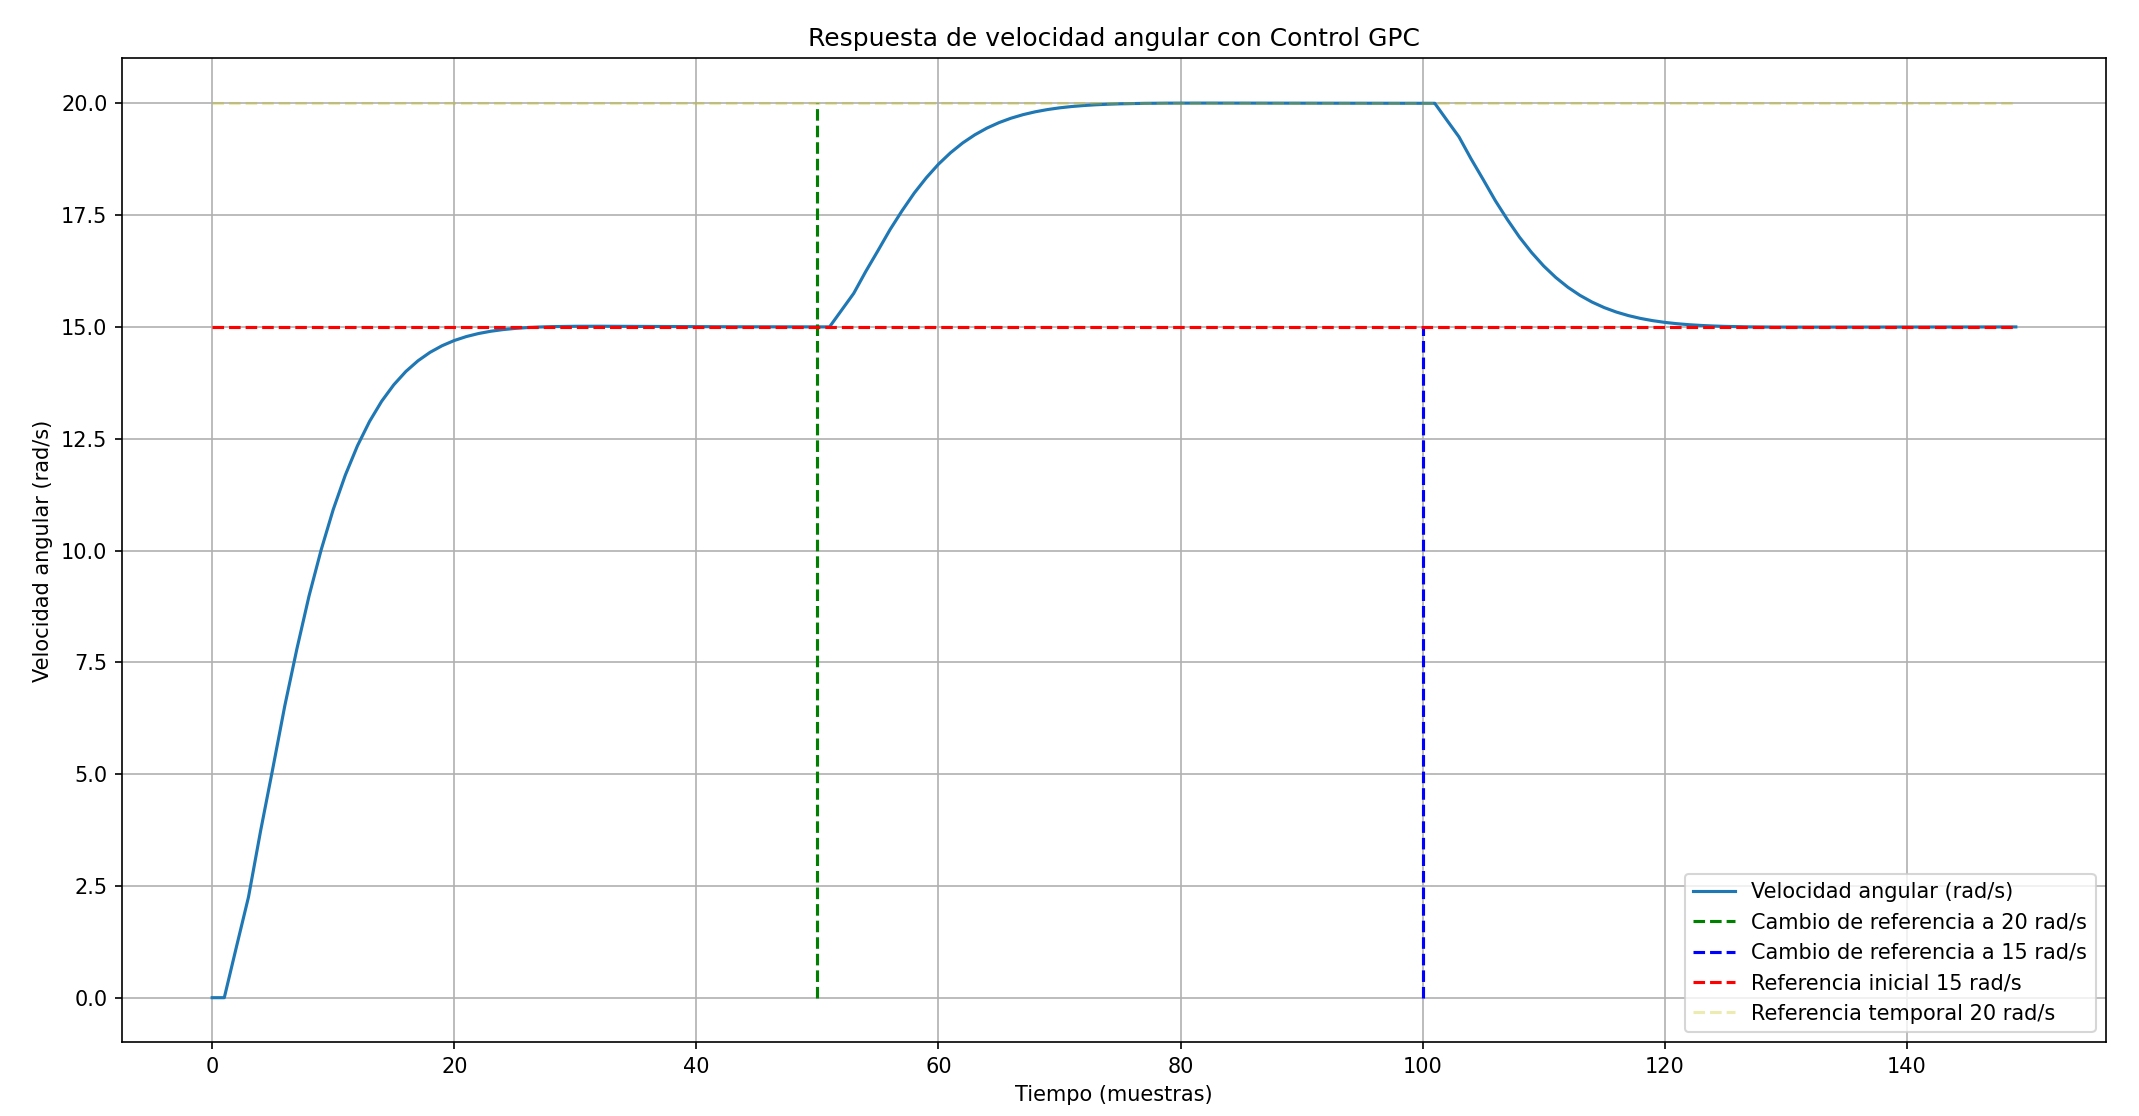
\includegraphics[width=1\linewidth]{imagen_1.png}
    \caption{Respuesta de la velocidad angular en $[rad/seg]$ para unos valores de las matrices de peso $Q = 9$ y $R= 0.5$. Los horizontes de predicción y control fueron de $\rho_1 = 5$  y $\rho_2 = 3$, respectivamente. }
    \label{fig:practico-1}
\end{figure}


\begin{figure}[H]
    \centering
    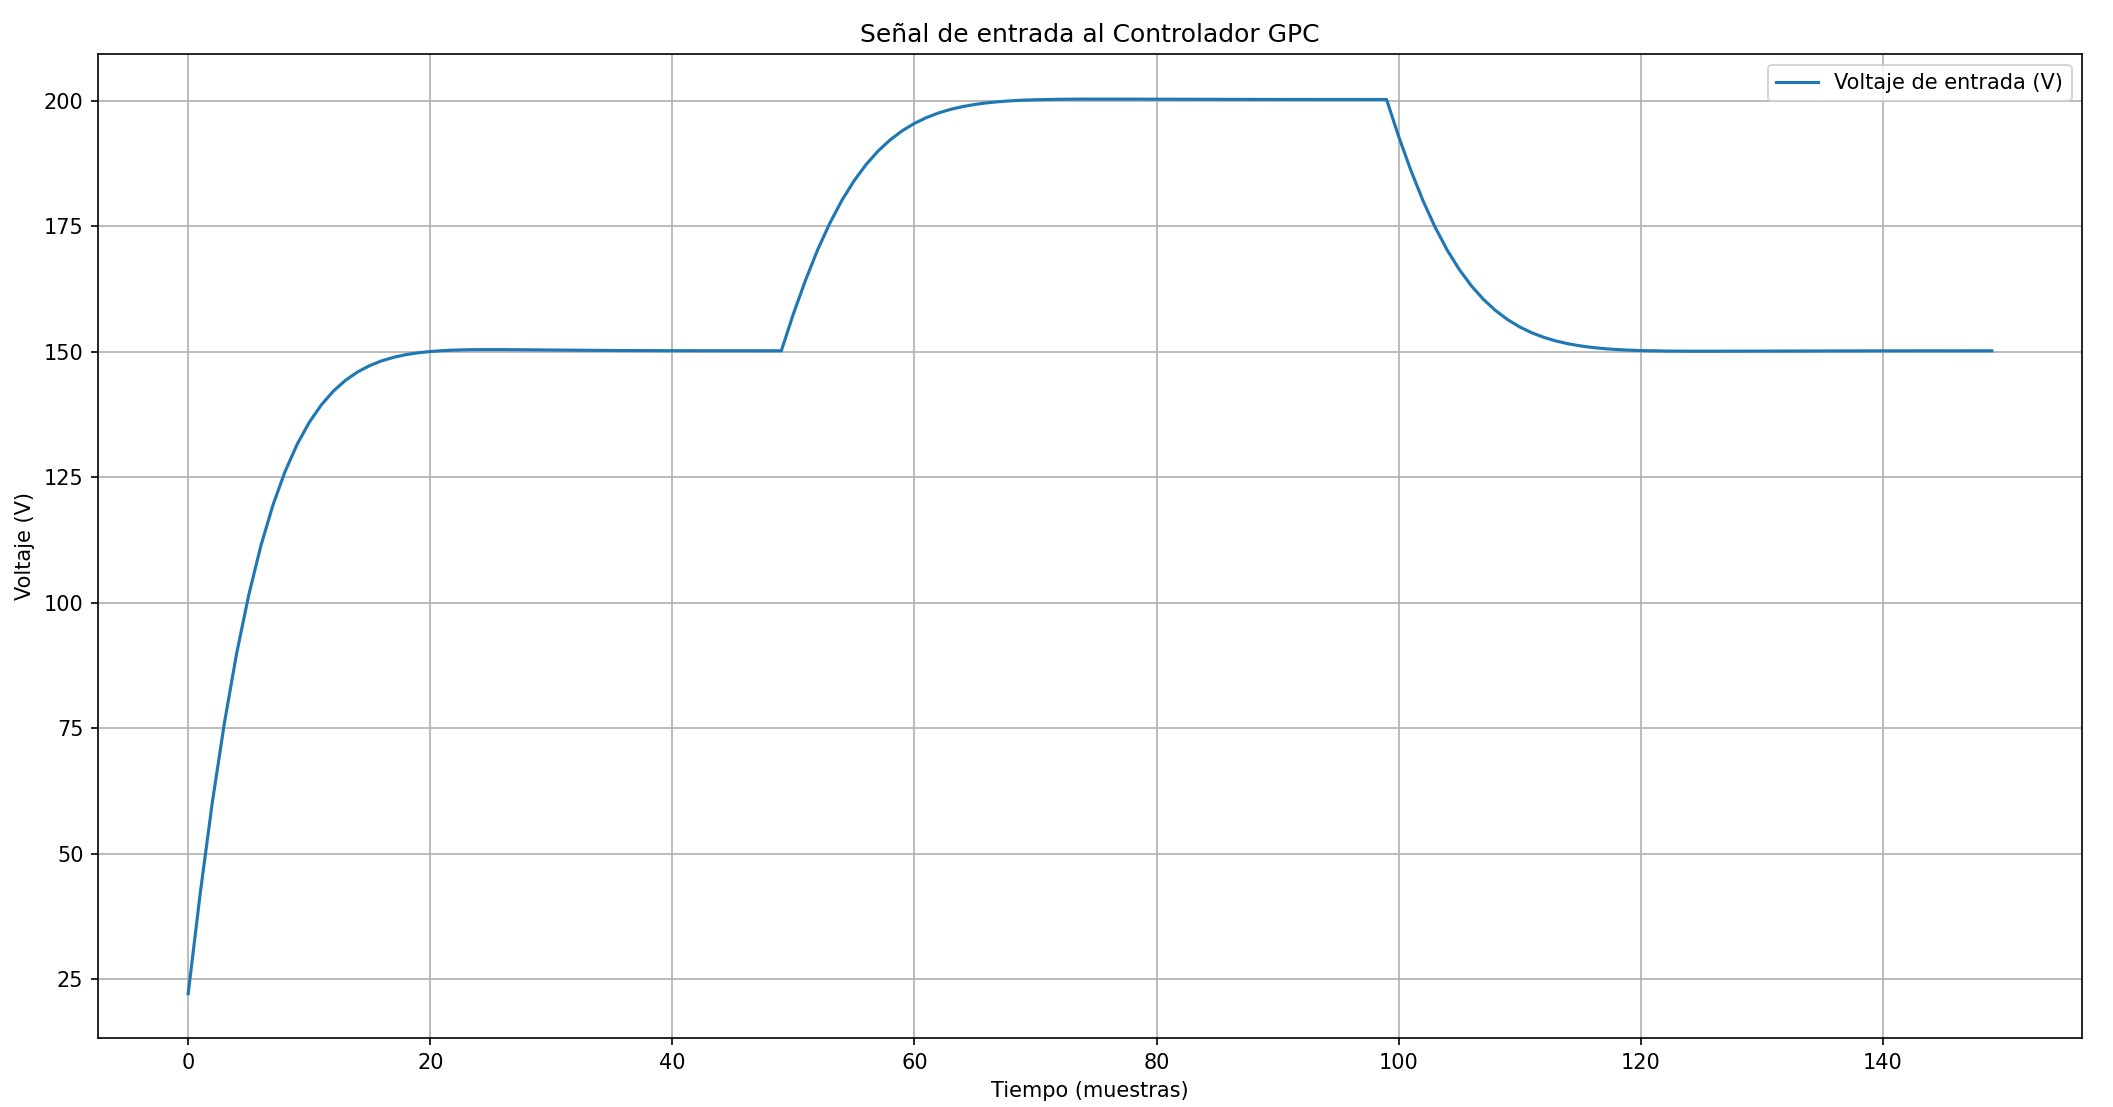
\includegraphics[width=1\linewidth]{imagen_2.png}
    \caption{Cambios de la entrada de voltaje en $[V]$ para valores de las matrices de peso $Q = 9$ y $R= 0.5$. Los horizontes de predicción y control fueron de $\rho_1 = 5$  y $\rho_2 = 3$, respectivamente. }
    \label{fig:practico-2}
\end{figure}

En la implementación y sintonización de un controlador predictivo generalizado (GPC), la matriz de ponderación del error \( Q \) juega un papel crucial en el equilibrio entre la rapidez de la respuesta transitoria y la suavidad de la acción de control. En las Figuras \ref{fig:practico-3} y \ref{fig:practico-4} se observa que al incrementar los valores de los elementos de \( Q \), se impone una mayor penalización sobre el error de seguimiento. Esto se traduce en una respuesta más agresiva del controlador, buscando minimizar la desviación de la trayectoria deseada con mayor determinación. Como consecuencia directa, se observa una reducción en el tiempo de establecimiento del estado transitorio, lo cual es indicativo de un sistema más reactivo a las discrepancias entre la salida predicha y la trayectoria de referencia.


\begin{figure}[H]
    \centering
    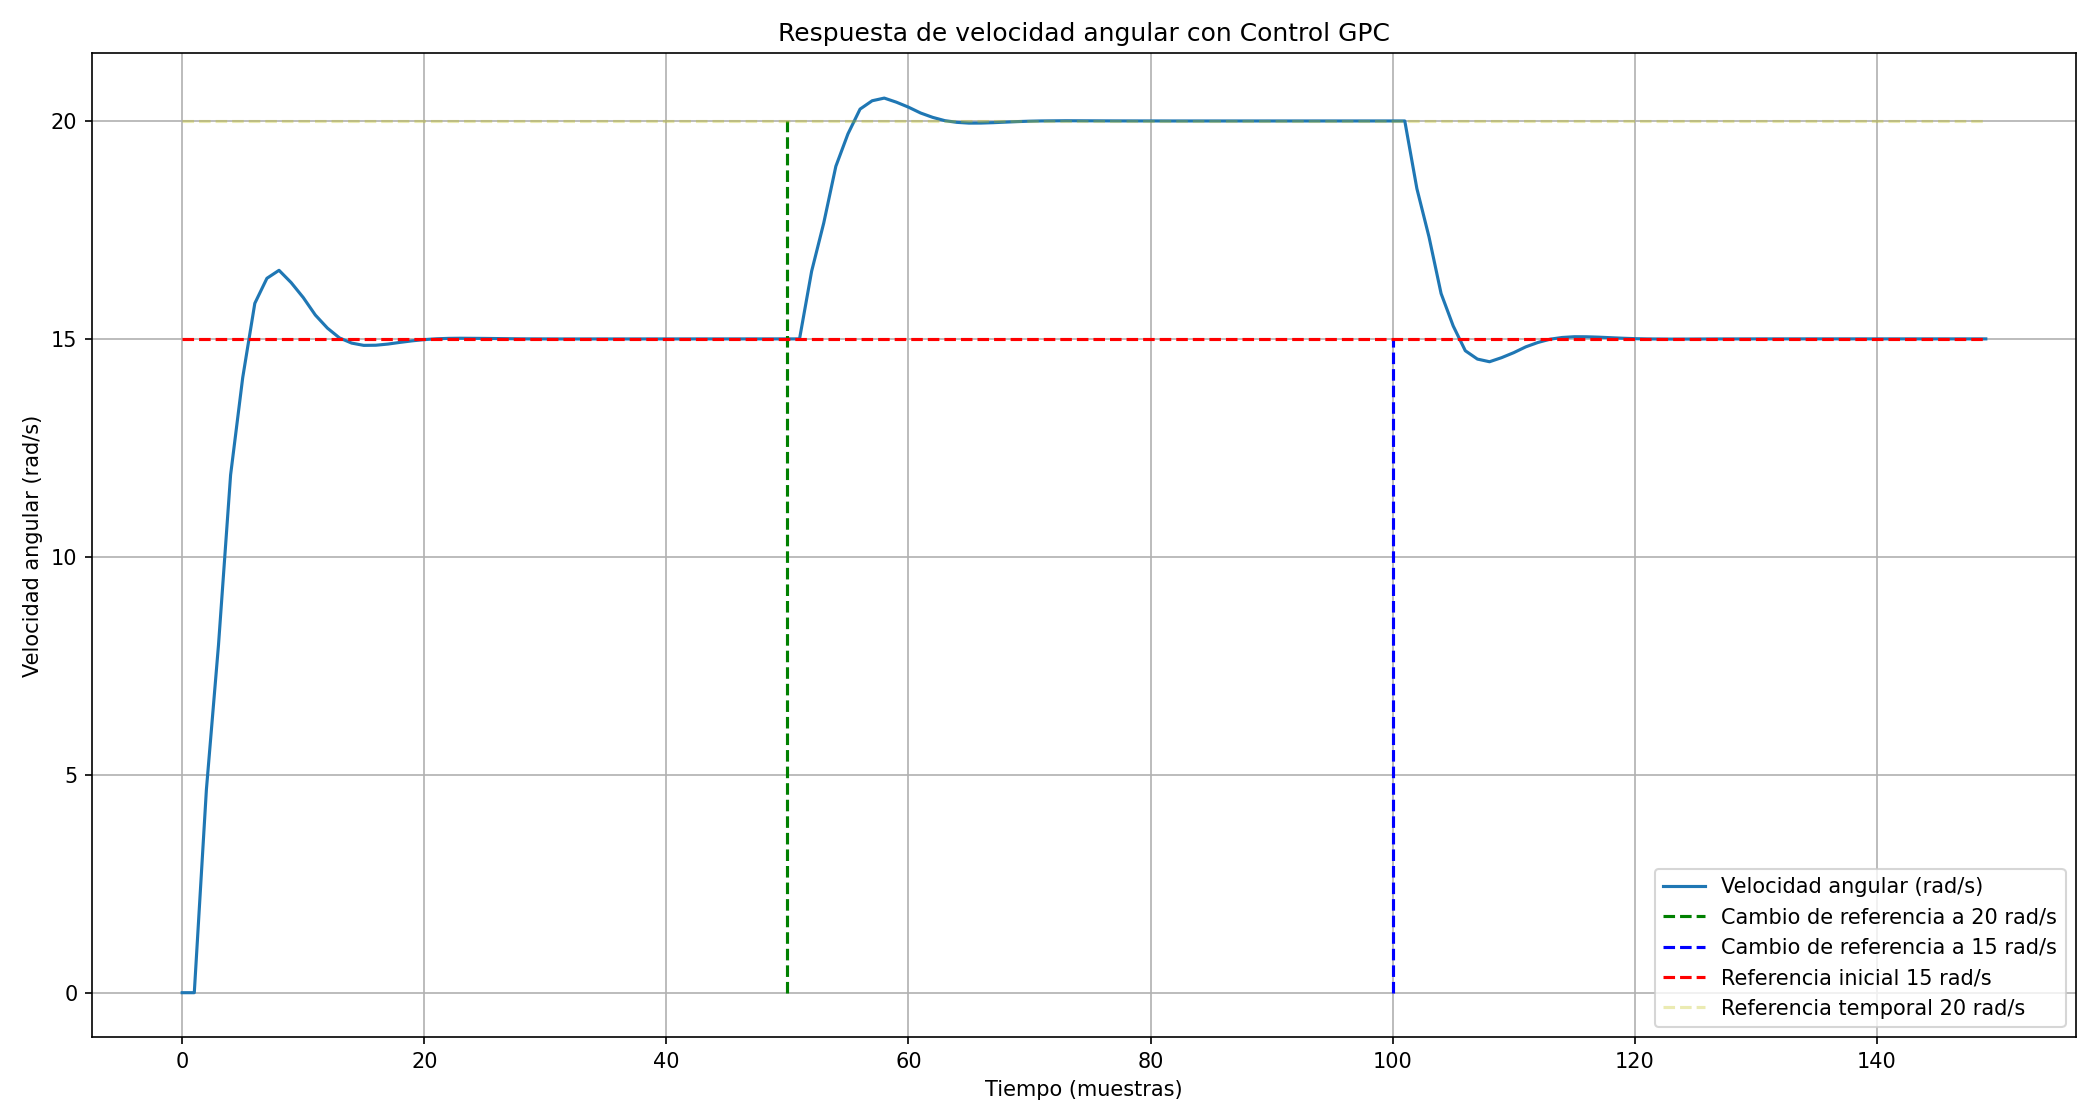
\includegraphics[width=1\linewidth]{imagen-3.png}
    \caption{Respuesta de la velocidad angular en $[rad/seg]$ para unos valores de las matrices de peso $Q = 50$ y $R= 0.5$. Los horizontes de predicción y control fueron de $\rho_1 = 5$  y $\rho_2 = 3$, respectivamente. }
    \label{fig:practico-3}
\end{figure}


Sin embargo, mantener un valor constante para la matriz de ponderación \( R \) asociada a la acción de control, mientras se aumenta \( Q \), puede resultar en un comportamiento no deseado en términos de la calidad de la señal de control. En particular, los incrementos de control \( \Delta U \) tienden a ser menos suaves, ya que la priorización del seguimiento de referencia sobre la moderación de la acción de control se ve reforzada. Esta condición puede conducir a un sistema que responde con movimientos más bruscos y menos graduales, lo cual es especialmente palpable en aplicaciones donde la suavidad de operación es primordial.

Además, un incremento significativo en los valores de \( Q \) puede introducir un comportamiento de sobreimpulso en la velocidad angular del sistema, donde se excede la referencia establecida. Este efecto es particularmente evidente en la presencia de un sobreimpulso que sobrepasa el valor deseado de la referencia, lo que demuestra una compensación excesiva en el esfuerzo por minimizar el error. Tal fenómeno es una manifestación de la dinámica más agresiva impuesta por un \( Q \) elevado, que si bien acelera la corrección del error, también puede comprometer la estabilidad y el rendimiento óptimo del sistema.


\begin{figure}[H]
    \centering
    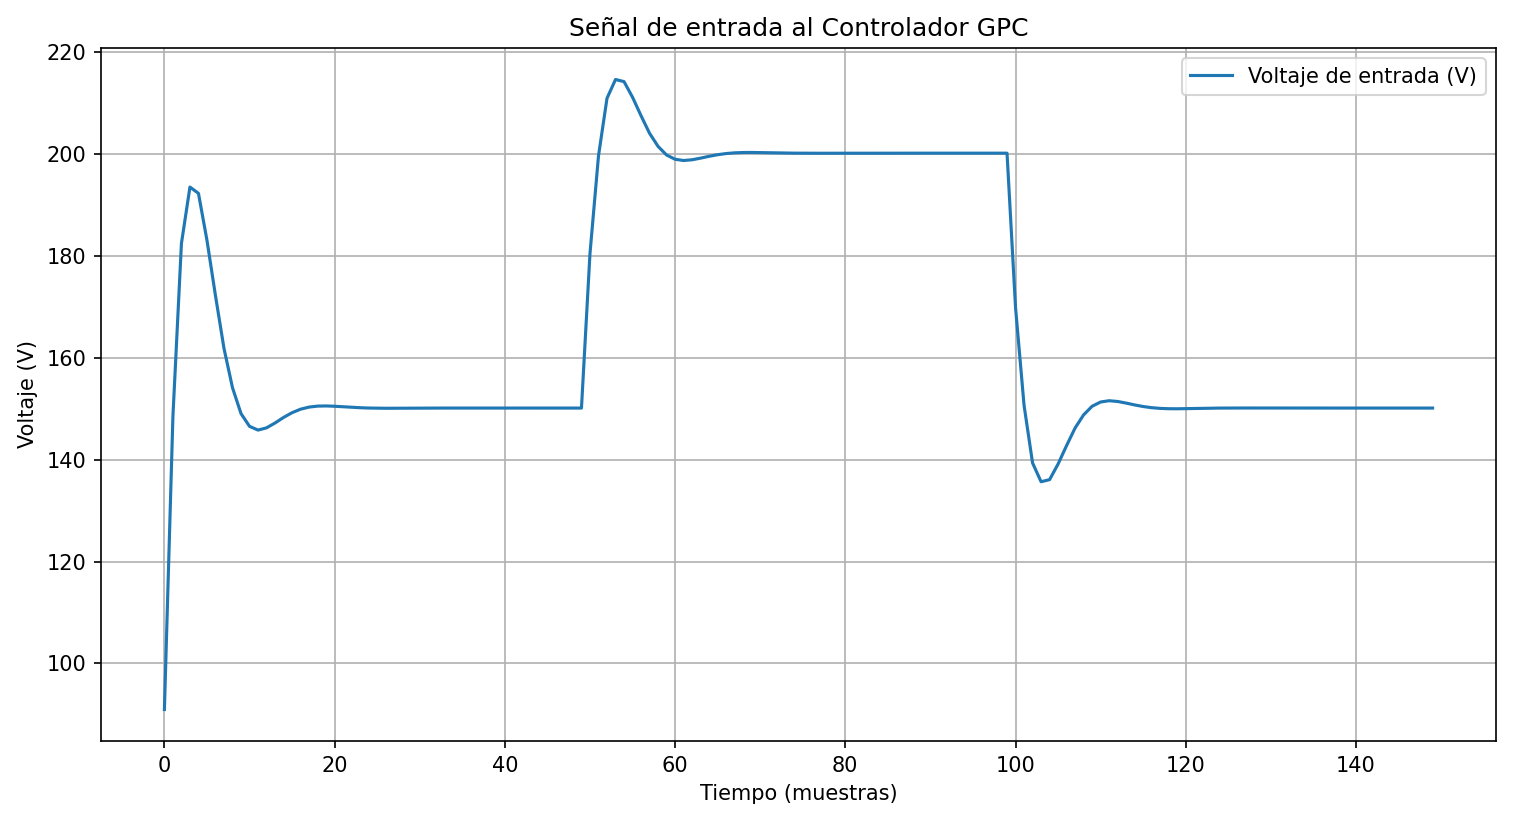
\includegraphics[width=1\linewidth]{imagen-4.png}
    \caption{Cambios de la entrada de voltaje en $[V]$ para unos valores de las matrices de peso $Q = 50$ y $R= 0.5$. Los horizontes de predicción y control fueron de $\rho_1 = 5$  y $\rho_2 = 3$, respectivamente. }
    \label{fig:practico-4}
\end{figure}

Como se ilustra en las Figuras \ref{fig:practico-5} y \ref{fig:practico-6}, un incremento en los valores de los pesos asociados a la matriz \( R \) provoca una extensión en los periodos de estado transitorio, reflejando un aumento en el tiempo que la velocidad angular, medida en \([rad/s]\), requiere para alcanzar el estado estacionario. Este fenómeno se atribuye a que una mayor ponderación en \( R \) induce una respuesta más cautelosa del controlador, priorizando la suavidad de la señal de control sobre la rapidez de seguimiento de la referencia.

Además, se observa que la señal de voltaje correspondiente al control de entrada adopta un perfil más suave. Esta característica es ventajosa en la práctica, ya que evita los sobreimpulsos en el voltaje que podrían ocasionar daños a los componentes electrónicos asociados al sistema de control.

\begin{figure}[H]
    \centering
    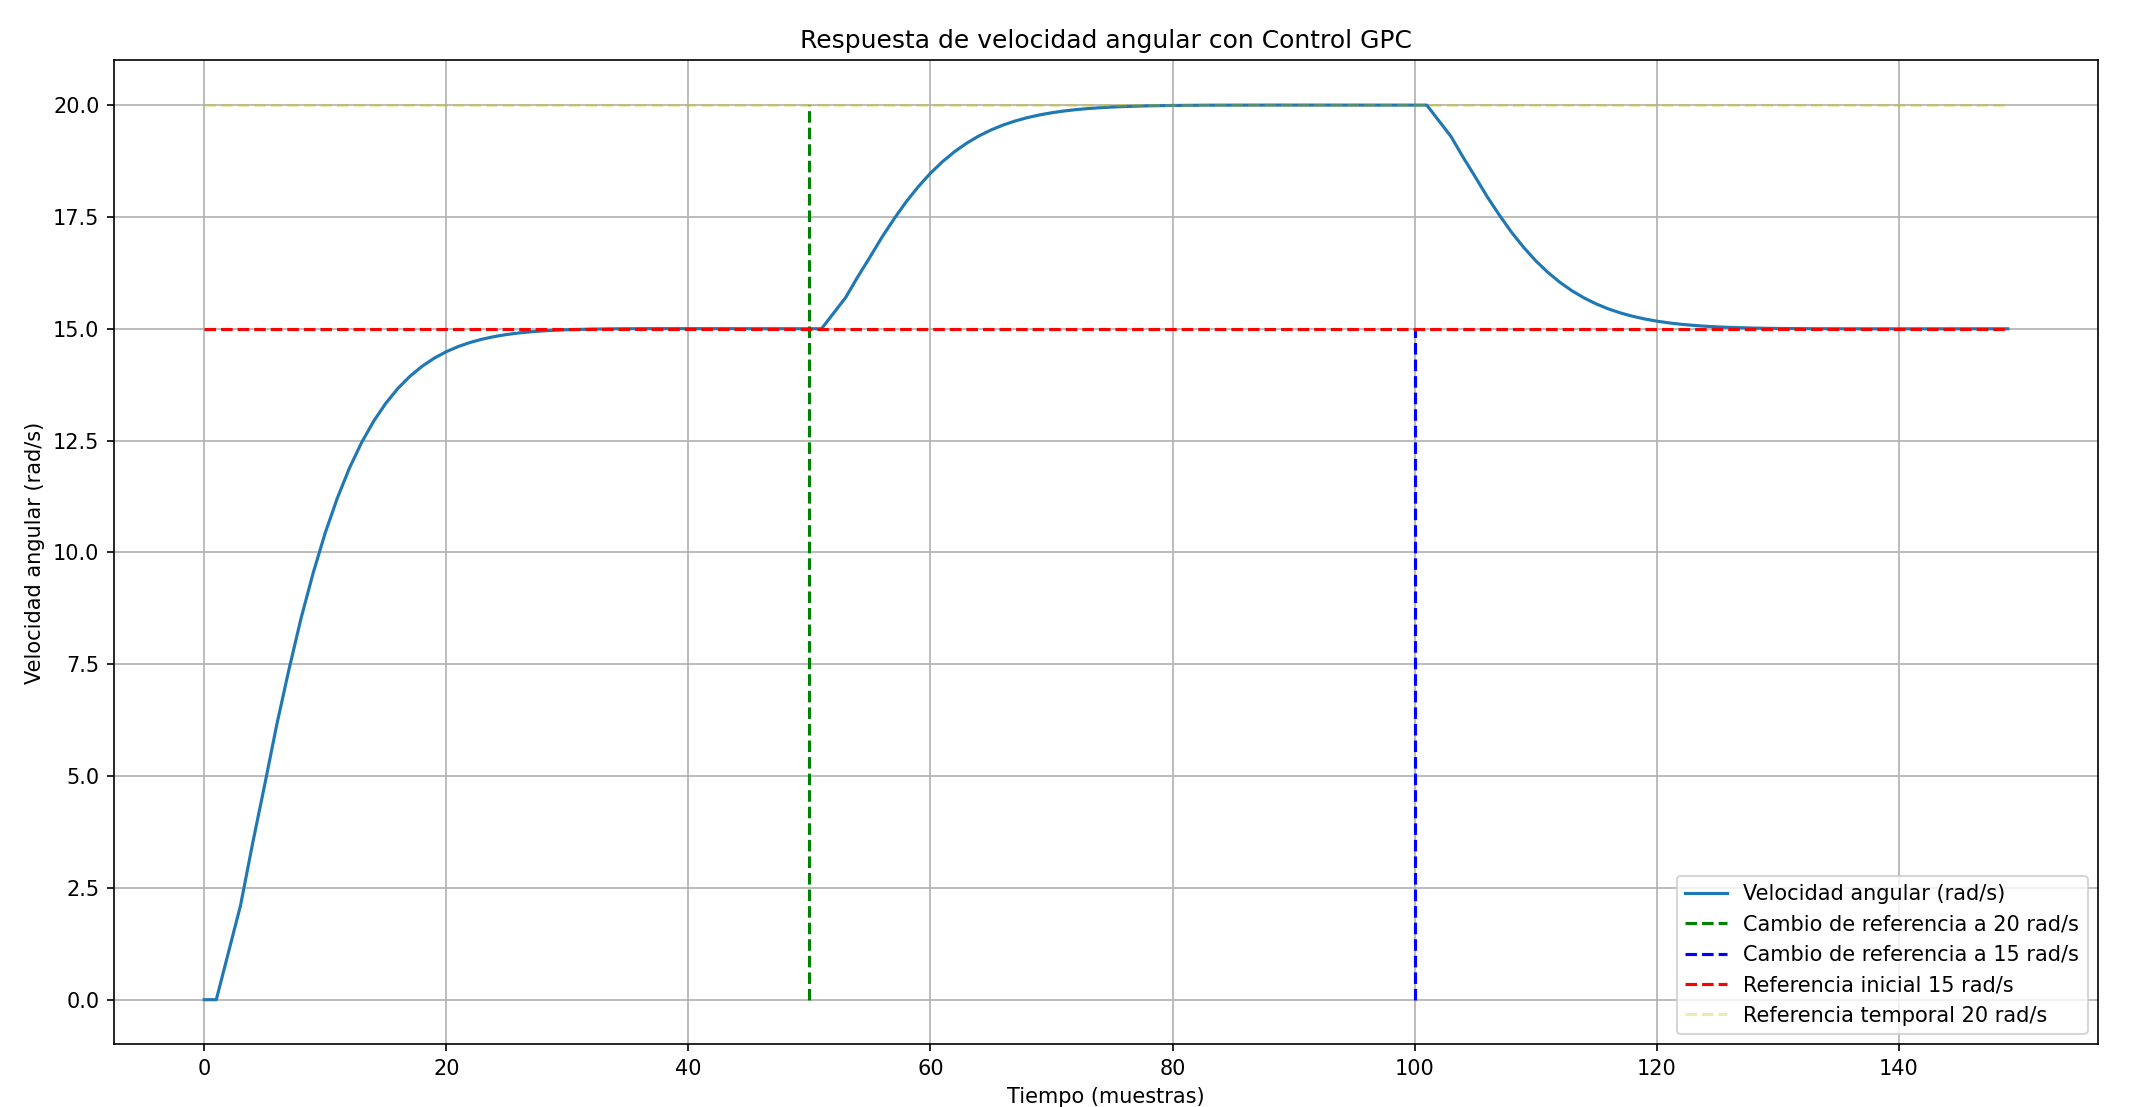
\includegraphics[width=1\linewidth]{imagen-7.png}
    \caption{Respuesta de la velocidad angular en $[rad/seg]$ para unos valores de las matrices de peso $Q = 50$ y $R= 3$. Los horizontes de predicción y control fueron de $\rho_1 = 5$  y $\rho_2 = 3$, respectivamente. }
    \label{fig:practico-5}
\end{figure}


\begin{figure}[H]
    \centering
    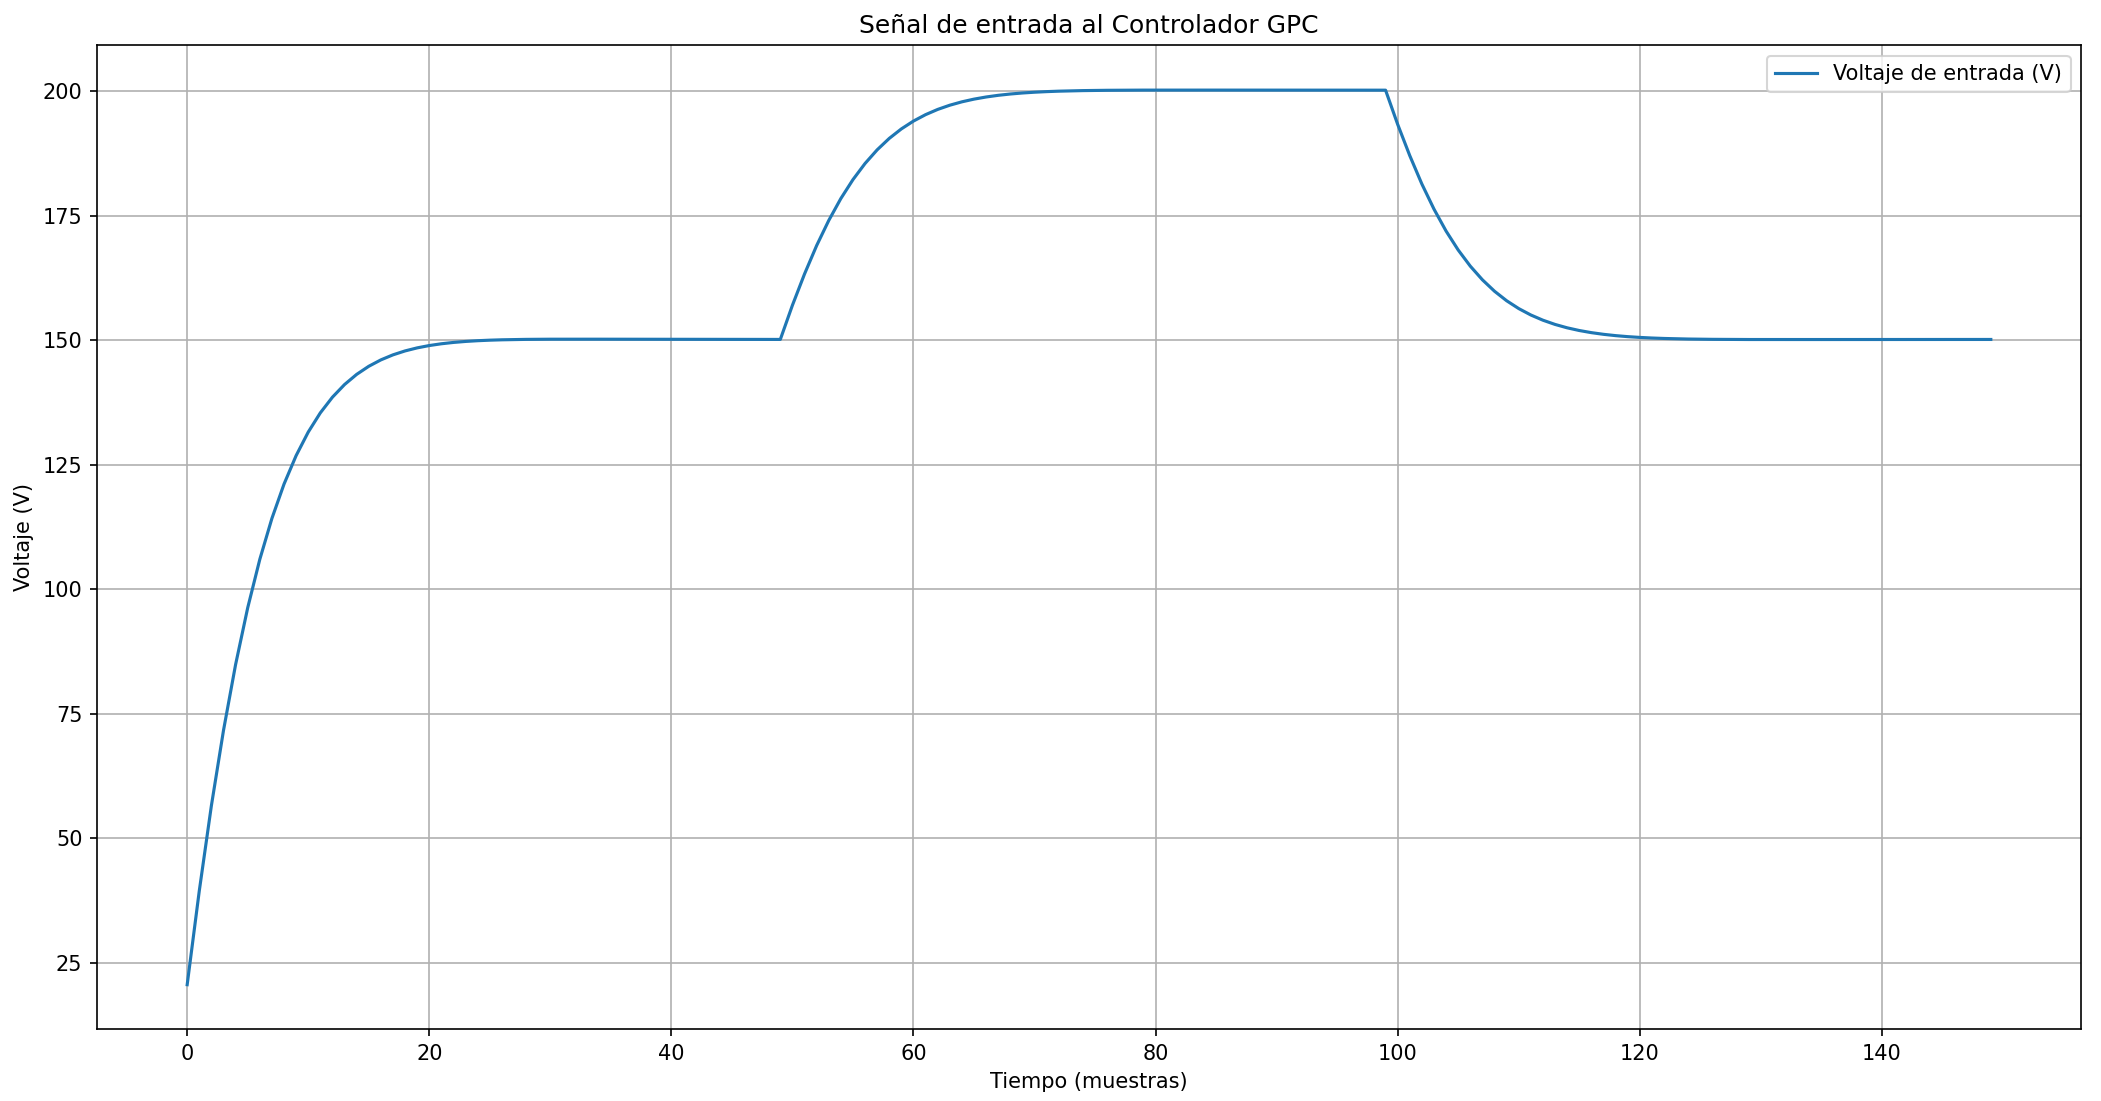
\includegraphics[width=1\linewidth]{imagen 8.png}
    \caption{Cambios de la entrada de voltaje en $[V]$ para unos valores de las matrices de peso $Q = 50$ y $R= 3$. Los horizontes de predicción y control fueron de $\rho_1 = 5$  y $\rho_2 = 3$, respectivamente. }
    \label{fig:practico-6}
\end{figure}


Por otro lado, como se muestra en las Figuras \ref{fig:practico-7} y \ref{fig:practico-8}, la reducción de los valores de los pesos \( R \) conduce a una disminución notable en los tiempos de estado transitorio, acompañada, sin embargo, de un sobreimpulso en la velocidad angular. Este comportamiento más agresivo en la respuesta del sistema se manifiesta a través de señales de control con oscilaciones y picos más pronunciados, que, si bien logran una estabilización más rápida, pueden ser perjudiciales para la integridad del motor y otros componentes mecánicos, especialmente si la entrada de control es el voltaje.

\begin{figure}[H]
    \centering
    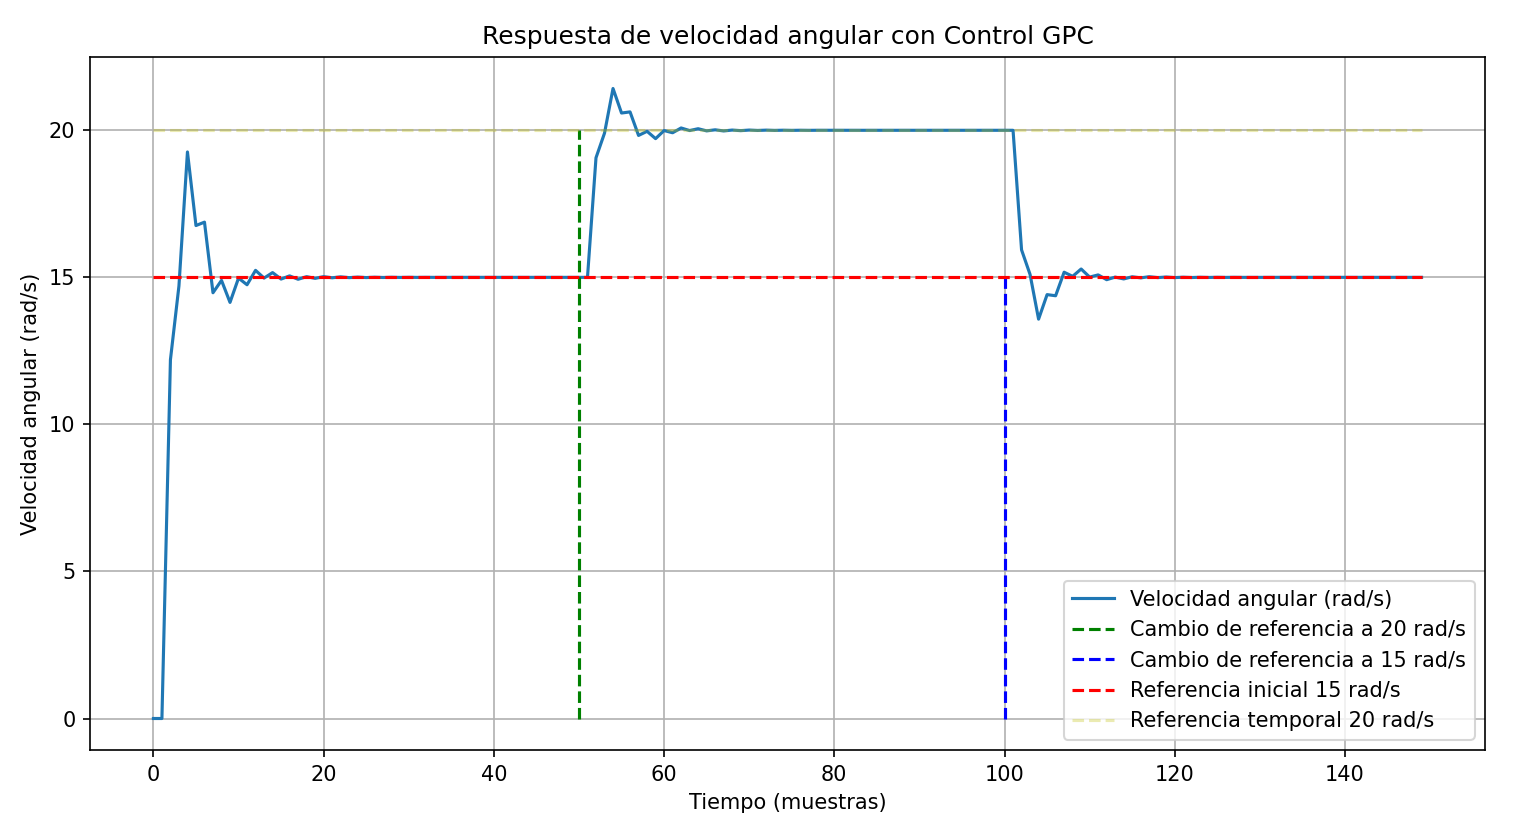
\includegraphics[width=1\linewidth]{imagen5.png}
    \caption{Respuesta de la velocidad angular en $[rad/seg]$ para unos valores de las matrices de peso $Q = 50$ y $R= 0.05$. Los horizontes de predicción y control fueron de $\rho_1 = 5$  y $\rho_2 = 3$, respectivamente. }
    \label{fig:practico-7}
\end{figure}


\begin{figure}[H]
    \centering
    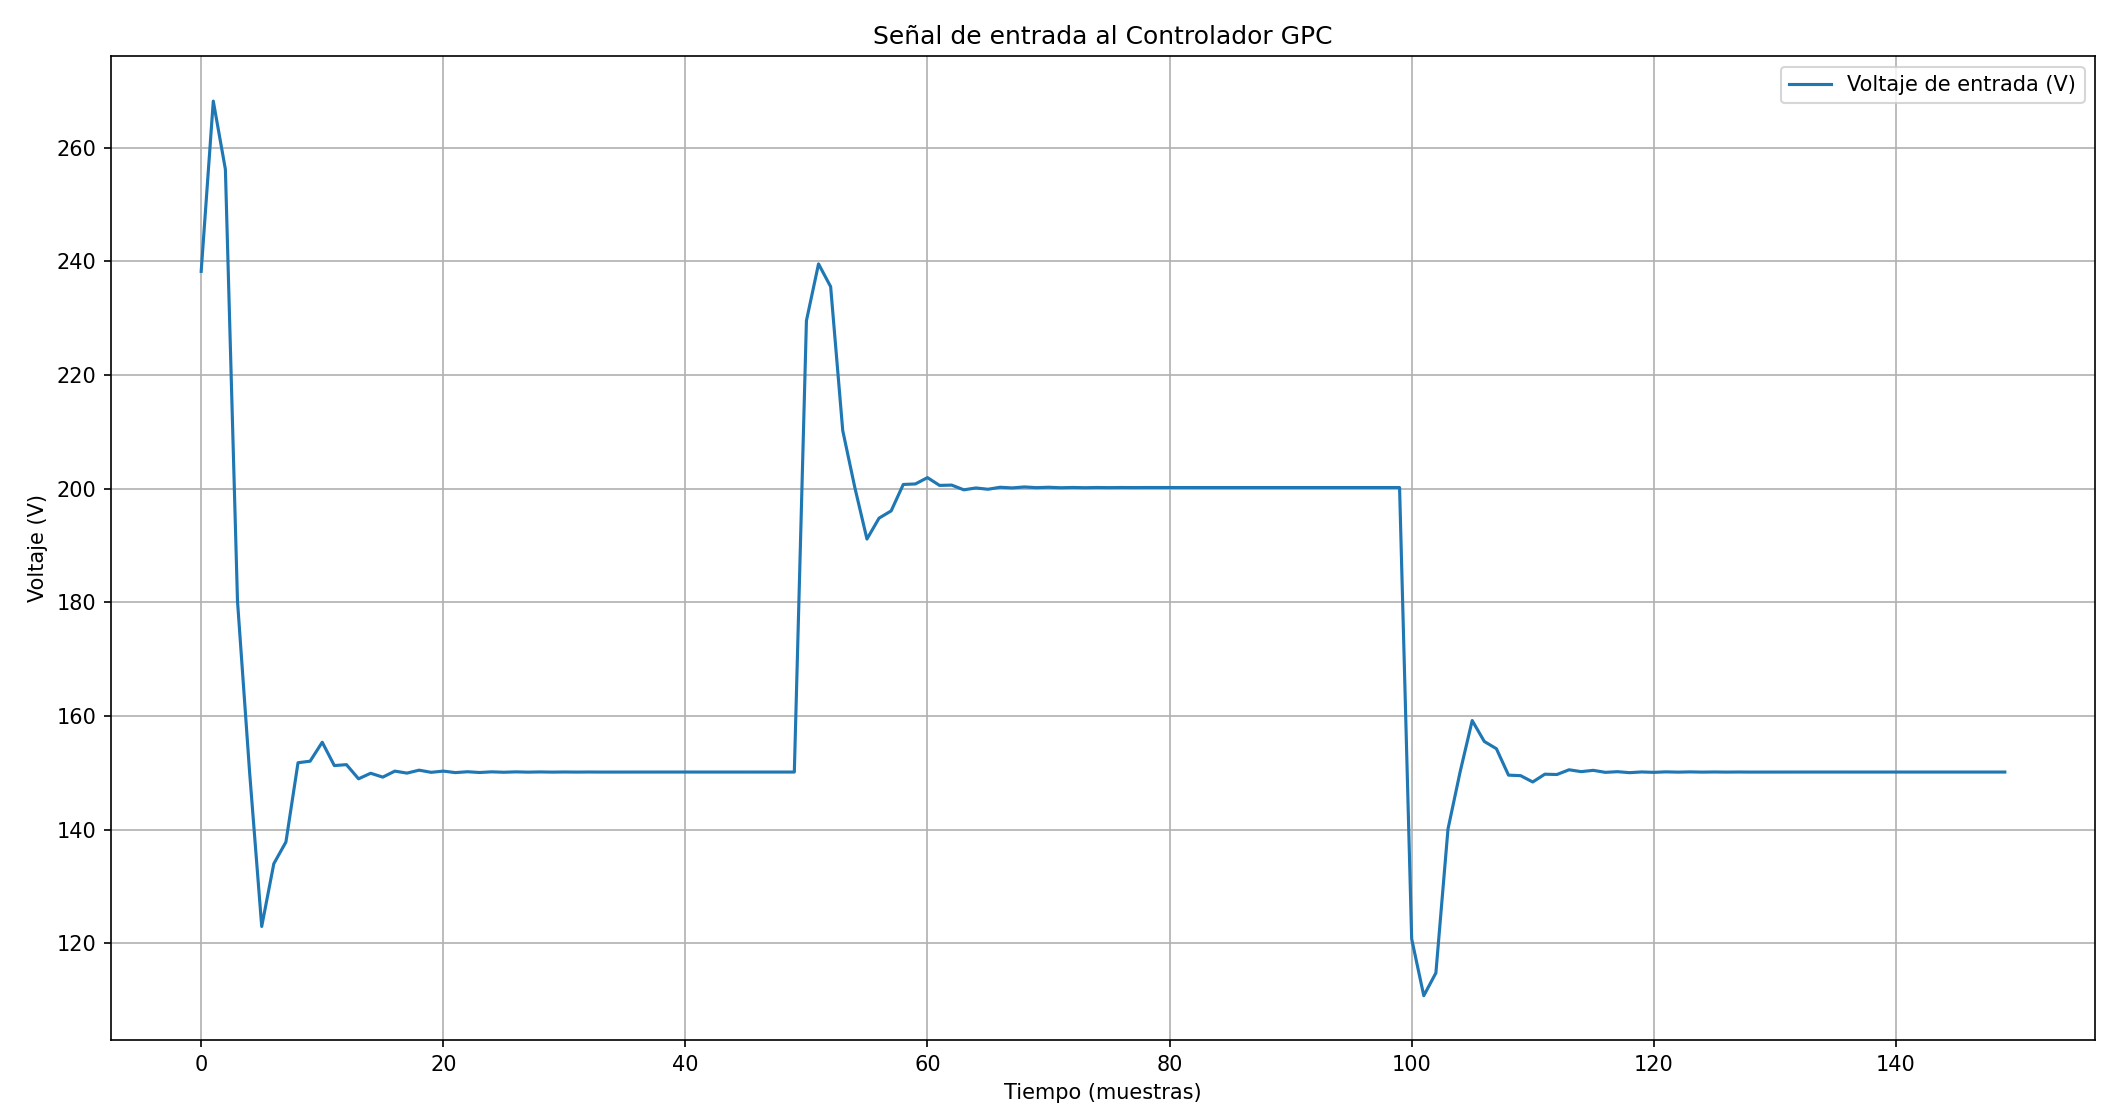
\includegraphics[width=1\linewidth]{imagen 6.png}
    \caption{Cambios de la entrada de voltaje en $[V]$ para unos valores de las matrices de peso $Q = 50$ y $R= 0.05$. Los horizontes de predicción y control fueron de $\rho_1 = 5$  y $\rho_2 = 3$, respectivamente. }
    \label{fig:practico-8}
\end{figure}



Este análisis describe la importancia de una cuidadosa selección de los valores dentro de la matriz \( R \) para el diseño del controlador predictivo generalizado (GPC). Ajustar adecuadamente \( R \) permite encontrar un equilibrio entre la protección de los componentes eléctricos y la eficiencia en la respuesta dinámica del sistema, factores ambos críticos para el funcionamiento seguro y efectivo en aplicaciones prácticas.


% An example of a floating figure using the graphicx package.
% Note that \label must occur AFTER (or within) \caption.
% For figures, \caption should occur after the \includegraphics.
% Note that IEEEtran v1.7 and later has special internal code that
% is designed to preserve the operation of \label within \caption
% even when the captionsoff option is in effect. However, because
% of issues like this, it may be the safest practice to put all your
% \label just after \caption rather than within \caption{}.
%
% Reminder: the "draftcls" or "draftclsnofoot", not "draft", class
% option should be used if it is desired that the figures are to be
% displayed while in draft mode.
%
%\begin{figure}[!t]
%\centering
%\includegraphics[width=2.5in]{myfigure}
% where an .eps filename suffix will be assumed under latex, 
% and a .pdf suffix will be assumed for pdflatex; or what has been declared
% via \DeclareGraphicsExtensions.
%\caption{Simulation results for the network.}
%\label{fig_sim}
%\end{figure}

% Note that the IEEE typically puts floats only at the top, even when this
% results in a large percentage of a column being occupied by floats.


% An example of a double column floating figure using two subfigures.
% (The subfig.sty package must be loaded for this to work.)
% The subfigure \label commands are set within each subfloat command,
% and the \label for the overall figure must come after \caption.
% \hfil is used as a separator to get equal spacing.
% Watch out that the combined width of all the subfigures on a 
% line do not exceed the text width or a line break will occur.
%
%\begin{figure*}[!t]
%\centering
%\subfloat[Case I]{\includegraphics[width=2.5in]{box}%
%\label{fig_first_case}}
%\hfil
%\subfloat[Case II]{\includegraphics[width=2.5in]{box}%
%\label{fig_second_case}}
%\caption{Simulation results for the network.}
%\label{fig_sim}
%\end{figure*}
%
% Note that often IEEE papers with subfigures do not employ subfigure
% captions (using the optional argument to \subfloat[]), but instead will
% reference/describe all of them (a), (b), etc., within the main caption.
% Be aware that for subfig.sty to generate the (a), (b), etc., subfigure
% labels, the optional argument to \subfloat must be present. If a
% subcaption is not desired, just leave its contents blank,
% e.g., \subfloat[].


% An example of a floating table. Note that, for IEEE style tables, the
% \caption command should come BEFORE the table and, given that table
% captions serve much like titles, are usually capitalized except for words
% such as a, an, and, as, at, but, by, for, in, nor, of, on, or, the, to
% and up, which are usually not capitalized unless they are the first or
% last word of the caption. Table text will default to \footnotesize as
% the IEEE normally uses this smaller font for tables.
% The \label must come after \caption as always.
%
%\begin{table}[!t]
%% increase table row spacing, adjust to taste
%\renewcommand{\arraystretch}{1.3}
% if using array.sty, it might be a good idea to tweak the value of
% \extrarowheight as needed to properly center the text within the cells
%\caption{An Example of a Table}
%\label{table_example}
%\centering
%% Some packages, such as MDW tools, offer better commands for making tables
%% than the plain LaTeX2e tabular which is used here.
%\begin{tabular}{|c||c|}
%\hline
%One & Two\\
%\hline
%Three & Four\\
%\hline
%\end{tabular}
%\end{table}


% Note that the IEEE does not put floats in the very first column
% - or typically anywhere on the first page for that matter. Also,
% in-text middle ("here") positioning is typically not used, but it
% is allowed and encouraged for Computer Society conferences (but
% not Computer Society journals). Most IEEE journals/conferences use
% top floats exclusively. 
% Note that, LaTeX2e, unlike IEEE journals/conferences, places
% footnotes above bottom floats. This can be corrected via the
% \fnbelowfloat command of the stfloats package.


\section{Conclusión}
En el presente trabajo se logró desarrollar una estrategia de control GPC para un motor DC. La selección cuidadosa y el ajuste fino de las matrices de ponderación de error \( Q \) y control \( R \) son esenciales para lograr una respuesta de control equilibrada. Es imperativo considerar la interacción entre \( Q \) y \( R \) para garantizar que se alcancen los objetivos de desempeño sin incurrir en comportamientos indeseables que puedan afectar adversamente al sistema o al proceso bajo control.



% if have a single appendix:
%\appendix[Proof of the Zonklar Equations]
% or
%\appendix  % for no appendix heading
% do not use \section anymore after \appendix, only \section*
% is possibly needed

% use appendices with more than one appendix
% then use \section to start each appendix
% you must declare a \section before using any
% \subsection or using \label (\appendices by itself
% starts a section numbered zero.)
%


%\appendices
%\section{Proof of the First Zonklar Equation}
%Appendix one text goes here.

% you can choose not to have a title for an appendix
% if you want by leaving the argument blank
%\section{}
%Appendix two text goes here.


% use section* for acknowledgment
%\section*{Acknowledgment}


%The authors would like to thank...


% Can use something like this to put references on a page
% by themselves when using endfloat and the captionsoff option.
\ifCLASSOPTIONcaptionsoff
  \newpage
\fi



% trigger a \newpage just before the given reference
% number - used to balance the columns on the last page
% adjust value as needed - may need to be readjusted if
% the document is modified later
%\IEEEtriggeratref{8}
% The "triggered" command can be changed if desired:
%\IEEEtriggercmd{\enlargethispage{-5in}}

% references section

% can use a bibliography generated by BibTeX as a .bbl file
% BibTeX documentation can be easily obtained at:
% http://mirror.ctan.org/biblio/bibtex/contrib/doc/
% The IEEEtran BibTeX style support page is at:
% http://www.michaelshell.org/tex/ieeetran/bibtex/
%\bibliographystyle{IEEEtran}
% argument is your BibTeX string definitions and bibliography database(s)
%\bibliography{IEEEabrv,../bib/paper}
%
% <OR> manually copy in the resultant .bbl file
% set second argument of \begin to the number of references
% (used to reserve space for the reference number labels box)
\begin{thebibliography}{1}

\bibitem{IEEEhowto:Abdelrauf}
A. A. ~Abdelrauf, M. Abdel-Geliel and E. Zakzouk, "Adaptive PID controller based on model predictive control," 2016 European Control Conference (ECC), Aalborg, Denmark, 2016, pp. 746-751, doi: 10.1109 /ECC.2016.7810378.

\bibitem{IEEEhowto:S}
Huang, ~S. (2002). Applied predictive control. Springer.

\bibitem{IEEEhowto:Castanio}
S. ~Castanio, «Modelo de motor DC», Control Automático Educación, 22 de noviembre de 2023. https://controlautomaticoeducacion.com/analisis-de-sistemas/modelo-de-motor-dc/
\end{thebibliography}

% biography section
% 
% If you have an EPS/PDF photo (graphicx package needed) extra braces are
% needed around the contents of the optional argument to biography to prevent
% the LaTeX parser from getting confused when it sees the complicated
% \includegraphics command within an optional argument. (You could create
% your own custom macro containing the \includegraphics command to make things
% simpler here.)
%\begin{IEEEbiography}[{\includegraphics[width=1in,height=1.25in,clip,keepaspectratio]{mshell}}]{Michael Shell}
% or if you just want to reserve a space for a photo:

%\begin{IEEEbiography}{Michael Shell}
%Biography text here.
%\end{IEEEbiography}

% if you will not have a photo at all:
%\begin{IEEEbiographynophoto}{John Doe}
%Biography text here.
%\end{IEEEbiographynophoto}

% insert where needed to balance the two columns on the last page with
% biographies
%\newpage

%\begin{IEEEbiographynophoto}{Jane Doe}
%Biography text here.
%\end{IEEEbiographynophoto}

% You can push biographies down or up by placing
% a \vfill before or after them. The appropriate
% use of \vfill depends on what kind of text is
% on the last page and whether or not the columns
% are being equalized.

%\vfill

% Can be used to pull up biographies so that the bottom of the last one
% is flush with the other column.
%\enlargethispage{-5in}



% that's all folks
\end{document}


